%----------------------------------------------------------------------------------------
%	CONFIGURATIONS
%----------------------------------------------------------------------------------------

\documentclass[12pt,a4paper,oneside]{article}

\usepackage[utf8]{inputenc}
\usepackage{graphicx}
\usepackage{epstopdf}
\usepackage{natbib}
\usepackage{amsmath}
\usepackage{lipsum}
\usepackage{caption}
\usepackage{subcaption}
\usepackage[a4paper,left=2cm,right=2cm,top=2.5cm,bottom=2.5cm]{geometry}
\usepackage[noend]{algpseudocode}
\usepackage{algorithmicx}
\usepackage[Algoritmo]{algorithm}

%----------------------------------------------------------------------------------------
%	INFORMATION
%----------------------------------------------------------------------------------------

\title{Métodos de pesquisa no jogo de \textit{Sesqui}\\
  \vspace{0.1in}
  \large{Inteligência Artificial - Trabalho 2}
}

\author{Miguel Ferreira\footnote{Miguel Ferreira - 201304200}, Pedro Paredes\footnote{Pedro Paredes - 201205725}, DCC - FCUP}

\date{Abril 2015}

\renewcommand{\tablename}{Tabela}
\renewcommand{\figurename}{Figura}
\renewcommand{\refname}{Referências}

\begin{document}

\maketitle

%----------------------------------------------------------------------------------------
%	SECTION 1
%----------------------------------------------------------------------------------------

\section{Introdução}
\label{sec:intro}

A existência de jogos surge naturalmente em muitas situações do
quotidiano. Em economia uma interação entre duas ou mais entidades
competidoras é normalmente vista como um jogo onde cada uma tenta
maximizar o seu lucro ou proveito. Porém, qualquer situação onde haja
cooperação ou conflito pode ser modelada como um jogo e as técnicas a
aplicar são semelhantes. Pode-se dizer assim que o estudo de jogos é o
estudo de processos de decisão.

Neste relatório exploraremos um subconjunto muito específico de jogos,
nomeadamente jogos determinísticos, discretos, de informação completa
e \textit{zero-sum} (embora alguns dos métodos se apliquem a muitos
outros tipos de jogos). A última característica é talvez a mais
importante e o que diz, informalmente, é que ``a sorte de uns é a
desgraça de outros'', o que significa que os recursos do jogo são
contantes, ou seja, o ganho de um jogador é exatamente a perda dos
seus oponentes. Mais especificamente explorar-se-á o jogo
\textit{Sesqui}, que é um jogo de tabuleiro de 2 jogadores e que será
descrito com maior pormenor numa secção futura.

O objetivo do relatório é de estudar métodos que permitam jogar
competitivamente jogos como os descritos a cima. Sendo assim
exploram-se 3 métodos diferentes: o algoritmo \textit{Minimax}, o
algoritmo de \textit{Alpha-Beta Pruning} e a \textit{Monte Carlo Tree
  Search}.

O resto do relatório está organizado da seguinte forma. Na Secção
\ref{sec:algconc} apresentamos uma descrição teórica dos 3 métodos de
otimizações comuns a cada um. Na Secção \ref{sec:sesqui} apresenta-se
o jogo \textit{Sesqui}, alguns resultados relacionados assim como uma
motivação para a implementação. Na Secção \ref{sec:imp} descreve-se a
nossa implementação dos métodos da Secção \ref{sec:algconc} e como
foram usados, assim como as heurísticas aplicadas ao
\textit{Sesqui}. Na Secção \ref{sec:resdes} discutem-se os resultados
e o desempenho da implementação. Finalmente, na Secção \ref{sec:conc}
é feita uma nota final sobre o trabalho e o relatório.

%----------------------------------------------------------------------------------------
%	SECTION 2
%----------------------------------------------------------------------------------------

\section{Algoritmos e Conceitos de Pesquisa em Jogos \textit{zero-sum}}
\label{sec:algconc}

Existem várias maneiras de abordar um jogo. Para jogos mais simples
como o \textit{Nim} existe uma estratégia vencedora, para a maior
parte das posições iniciais, que se baseia num invariante do
jogo. Para jogos que sejam facilmente decompostos em subjogos
independentes, o teorema de \textit{Sprague-Grundy} pode ser usado
para obter uma estratégia. Para certos jogos, como o \textit{Connect
  Four} (conhecido em português pelo ``4 em linha'')
\cite{Allis:1988}, foram aplicados conhecimentos de combinatória para
resolver o jogo, ou seja, para obter uma estratégia vencedora do
jogo.

Porém, para a maior parte dos jogos, não é fácil obter resultados como
estes. É necessário assim recorrer a métodos exaustivos, que enumeram
os vários estados possíveis do jogo. Nesta secção descrevemos 3
métodos com este comportamento. A ideia geral deste métodos é de a
partir de uma configuração inicial enumerar as várias transições
possíveis com o objetivo de explorar o espaço de estados disponível
até chegar a posições terminais. Como este espaço de estados pode ser
demasiado extenso, recorrem-se a heurísticas para medir o valor de
configurações não terminais e assim efetua-se a pesquisa apenas até
uma certa profundidade.

Para simplificar a discussão nesta secção e nas próximas, introduzimos
alguns termos a usar. Um estado de um jogo é chamado de configuração
ou tabuleiro. O valor da função heurística para um determinado
tabuleiro é chamada da função utilidade. O \textit{payoff} é o valor
relativo de um tabuleiro (distinguimo-lo da função utilidade porque
consideramo-lo um valor teórico, enquanto que a função utilidade é um
valor empírico dado pela heurística). Na Subsecção \ref{ssec:mcts} é
descrito um algoritmo em árvore, por isso usa-se a notação padrão de
métodos de pesquisa (uma árvore cujos elementos são nós, o nó inicial
é a raiz e os nós mais profundos são as folhas \ldots).

\subsection{O Teorema e o Algoritmo Minimax}

%Cite something about Von Neumann
O teorema de Minimax garante a existência de um valor $V$ e uma estratégia para cada jogador de um jogo \emph{zero-sum}, de maneira a que o primeiro jogador tenha um \emph{payoff} ótimo de $V$ e o segundo um \emph{payoff} ótimo de $-V$, dadas as estratégias dos seus oponentes.

O nome ``Minimax'' resulta da estratégia de minimizar o \emph{payoff} máximo do jogador oponente e, dado a soma-zero do jogo, maximizar o próprio \emph{payoff}.

O algoritmo de Minimax aplica a ideia descrita pelo teorema através de uma busca em profundidade, devolvendo assim o melhor \emph{payoff} para o um dado estado do jogo. Este algoritmo tem complexidade exponencial de $O(b^{h})$, sendo $b$ o fator de ramificação do jogo e $h$ um limite superior do número máximo de jogadas.

\begin{algorithm}
\begin{algorithmic}
\Function{Minimax}{$Node$, $Player$} \Comment{Devolve o valor minimax do melhor nó seguinte}
  \If{\Call{Terminal}{$Node$}} \Return{\Call{Value}{$Node$}}
  \EndIf
  \If{$Player=min$}
      \State $best \gets \infty$
      \For{$son$ in \Call{Successors}{$Node$}}
          \State $next \gets$ \Call{Minimax}{$son$, $max$}
          \State $best \gets$ \Call{Min}{$best$, $next$}
      \EndFor
  \ElsIf{$Player=max$}
      \State $best \gets -\infty$
      \For{$son$ in \Call{Successors}{$Node$}}
          \State $next \gets$ \Call{Minimax}{$son$, $min$}
          \State $best \gets$ \Call{Max}{$best$, $next$}
      \EndFor
  \EndIf
  \State\Return{$best$} 
\EndFunction
\end{algorithmic}
\caption{Minimax}
\end{algorithm}

\subsubsection{O Negamax}

O algoritmo Negamax é uma variante simplificada do Minimax para jogos que verificam uma simetria entre os valores do estado para cada um dos jogadores. Sendo assim, é possível minimizar ou maximizar valores do oponente através da negação do valor Negamax da jogada seguinte.

\begin{algorithm}
\begin{algorithmic}
\Function{Negamax}{$Node$} \Comment{Devolve o valor do melhor nó seguinte}
  \If{\Call{Terminal}{$Node$}} \Return{\Call{Value}{$Node$}}
  \EndIf
  \State $best \gets -\infty$
  \For{$son$ in \Call{Successors}{$Node$}}
      \State $next \gets -$\Call{Negamax}{$son$}
      \State $best \gets$ \Call{Max}{$best$, $next$}
  \EndFor
  \State\Return{$best$} 
\EndFunction
\end{algorithmic}
\caption{Negamax}
\end{algorithm}

\subsection{O Método \textit{Alpha-Beta Pruning}}

O algoritmo \emph{Alpha-Beta Pruning} é uma versão otimizada do Minimax que devolve o valor correto sem percorrer necessariamente a árvore completa. Esta otimização consiste em não expandir nós que tenham um valor pior que outros já vistos anteriormente e efetivamente reduzir a árvore de pesquisa.

O nome ``Alpha-Beta'' deve-se ao uso de duas variáveis que, respetivamente, espeficicam o limite inferior e superior dos valores de nós que devem ser expandidos\cite{Russell:AI:2003}. A variável $\alpha$ guarda o valor do melhor para o jogador ``max'' e $\beta$ guarda o melhor valor para o jogador ``min''.

Uma limitação deste algoritmo é a dependência da ordem ``correta'' na análise dos nós sucessores. Se a lista sucessores for gerada de forma a que os nós que terão pior valor sejam expandidos primeiro, este algoritmo terá de percorrer a árvore completa.

\begin{algorithm}
\begin{algorithmic}
\Function{Alpha-Beta}{$Node$, $Player$, $\alpha$, $\beta$}
  \If{\Call{Terminal}{$Node$}} \Return{\Call{Value}{$Node$}}
  \EndIf
  \If{$Player=min$}
      \State $best \gets \infty$
      \For{$son$ in \Call{Successors}{$Node$}}
          \State $next \gets$ \Call{Alpha-Beta}{$son$, $max$, $\alpha$, $\beta$}
          \State $best \gets$ \Call{Min}{$best$, $next$}
          \If{$best \leq \alpha$}
              \State\Return{$best$}
          \EndIf
          \State $\beta \gets$ \Call{Min}{$\beta$, $best$}
      \EndFor
  \ElsIf{$Player=max$}
      \State $best \gets -\infty$
      \For{$son$ in \Call{Successors}{$Node$}}
          \State $next \gets$ \Call{Alpha-Beta}{$son$, $min$, $\alpha$, $\beta$}
          \State $best \gets$ \Call{Max}{$best$, $next$}
          \If{$best \geq \beta$}
              \State\Return{$best$}
          \EndIf
          \State $\alpha \gets$ \Call{Max}{$\alpha$, $best$}
      \EndFor
  \EndIf
  \State\Return{$best$} 
\EndFunction
\end{algorithmic}
\caption{\emph{Alpha-Beta Pruning}}
\end{algorithm}

\subsubsection{Otimizações Comuns}

Existem várias otimizações aos algoritmos acima descritos. Um exemplo seria tabelas de transposição\footnote{do inglês: \emph{Transposition Tables}.} que permitem memorizar as posições pelas quais o algoritmo de busca adversarial já passou e os seus respetivos valores. Dessa forma, é possível evitar recalcular valores de nós já calculados noutros ramos.

Tabelas de transposição são especialmente benéficas em pesquisas iterativas, porém constituem um custo de memória elevado.

É possível otimizar o \emph{pruning} do \emph{Alpha-Beta} através de \emph{Aspiration Windows}. Este método consiste na previsão e utilização de um limite inferior e superior mais curto. Na eventualidade o resultado verdadeiro se encontrar fora desta janela é necessário refazer a pesquisa com um intervalo maior.

Parar a uma dada prufundidade máxima nem sempre é a melhor estratégia para um agente artificial, porque o nó terminal pode causar grandes mudanças de jogo e o agente não pode expandir os nós seguintes para poder decidir se é uma jogada boa ou não.
\emph{Quiescence} é uma melhoria à qualidade do resultado da pesquisa \emph{Alpha-Beta}, avaliando apenas movimentos que não causem grandes mudanças no jogo e expandindo os restantes.

%(http://chessprogramming.wikispaces.com/Alpha-Beta#Enhancements)
%(http://www.arimaa.com/arimaa/papers/ThomasJakl/bc-thesis.pdf Section 3.1)

%Tópicos: Transposition Table, Iterative Deepening, Aspiration Windows, Move ordering, Quiescence Search
%Referir: NegaScout

\newpage

\subsection{\textit{Monte Carlo Tree Search}}
\label{ssec:mcts}

O algoritmo de \textit{Monte Carlo Tree Search} (a partir de agora
referenciado como \texttt{MCTS}) surgiu graças ao jogo de
\textit{Go}. Depois de muitos desenvolvimentos no ramo de Inteligência
artificial e de vários jogos a terem programas competitivos, o
\textit{Go} continuou a ``fugir'' a estes desenvolvimentos e até tão
cedo como 1998 um jogador profissional era capaz de vencer o melhor
programa com um \textit{handicap} de até 30 peças (num tabuleiro de 19
por 19).  Em 2005, baseado num trabalho desenvolvido em
1993\cite{Brugmann:1993}, surgiu um novo algoritmo que obteve
resultados muito melhores do que até então, a \texttt{MCTS}. Desde
então que já sofreu muitos desenvolvimentos e várias otimizações e é o
algoritmo com melhor performance em \textit{Go} e além disso foi
aplicado a vários outros jogos (como o \textit{Hex}, o \textit{Arimaa}
e até \textit{Poker}).

A ideia base é a de usar simulações pseudoaleatórias (chamadas de
\textit{playouts}) de jogos a partir de cada posição e verificar
quantas levam a resultados vencedores. Porém, algumas jogadas
``merecem'' mais atenção do que outras e assim são exploradas mais
vezes de maneira a ter a informação mais detalhada possível. O
algoritmo pode ser descrito com os seguintes 4 passos, que são
executados iterativamente múltiplas vezes:

\begin{itemize}
  \item \textbf{Seleção}: A partir do nó raiz (que representa o
    tabuleiro inicial), selecionar filhos sucessivos até chegar a uma
    folha;
  \item \textbf{Expansão}: Se o nó folha selecionado não for final,
    expande-o, criando os seus filhos e construindo as suas
    propriedades;
  \item \textbf{Simulação}: Simula um jogo pseudoaleatório até atingir
    uma configuração final;
  \item \textbf{Propagação}: Propaga a informação da simulação pelo nó
    folha selecionado e todos os seus nós antecessores;
\end{itemize}

A Figura \ref{fig:mcts} ilustra este processo. Este método no limite
converge para o \textit{Minimax}, isto é, se o número de iterações das
4 fases for suficientemente alto. Na prática normalmente o algoritmo
sofre um \textit{plateau} dependendo das otimizações usadas.

Algumas vantagens deste método em relação aos anteriormente
apresentados. O primeiro é que é um algoritmo \textit{anytime}, ou
seja, que pode ser parado a qualquer altura. Para jogos onde o
controlo de tempo é importante, esta propriedade ajuda a gerir o
tempo. Depois, não é necessária nenhuma heurística para guiar o
algoritmo (embora seja útil usar-se como se verá na Subsecção
\ref{sec:mcopt}). Além disso, é gerada uma árvore assimétrica
naturalmente. Ao contrário de métodos como o \textit{Alpha-Beta} que
cortam jogadas que não parecem promissoras, a \texttt{MCTS} explora
mais as que parecem mais promissoras, dando origem assim a uma árvore
assimétrica.

Contudo, existem também algumas desvantagens. Primeiro é mais lenta
que a \textit{Alpha-Beta}. Para se obter um bom resultado é necessário
perder mais tempo, em média, do que na \textit{Alpha-Beta}. Outra
desvantagem é que a árvore de procura tem de ser mantida em memória, o
que introduz mais uma limitação possível ao algoritmo. Existem outras
desvantagens que foram mais notadas com a implementação do algoritmo e
que serão descritas na Secção \ref{sec:imp}.

\begin{figure}[!htb]
  \centering
  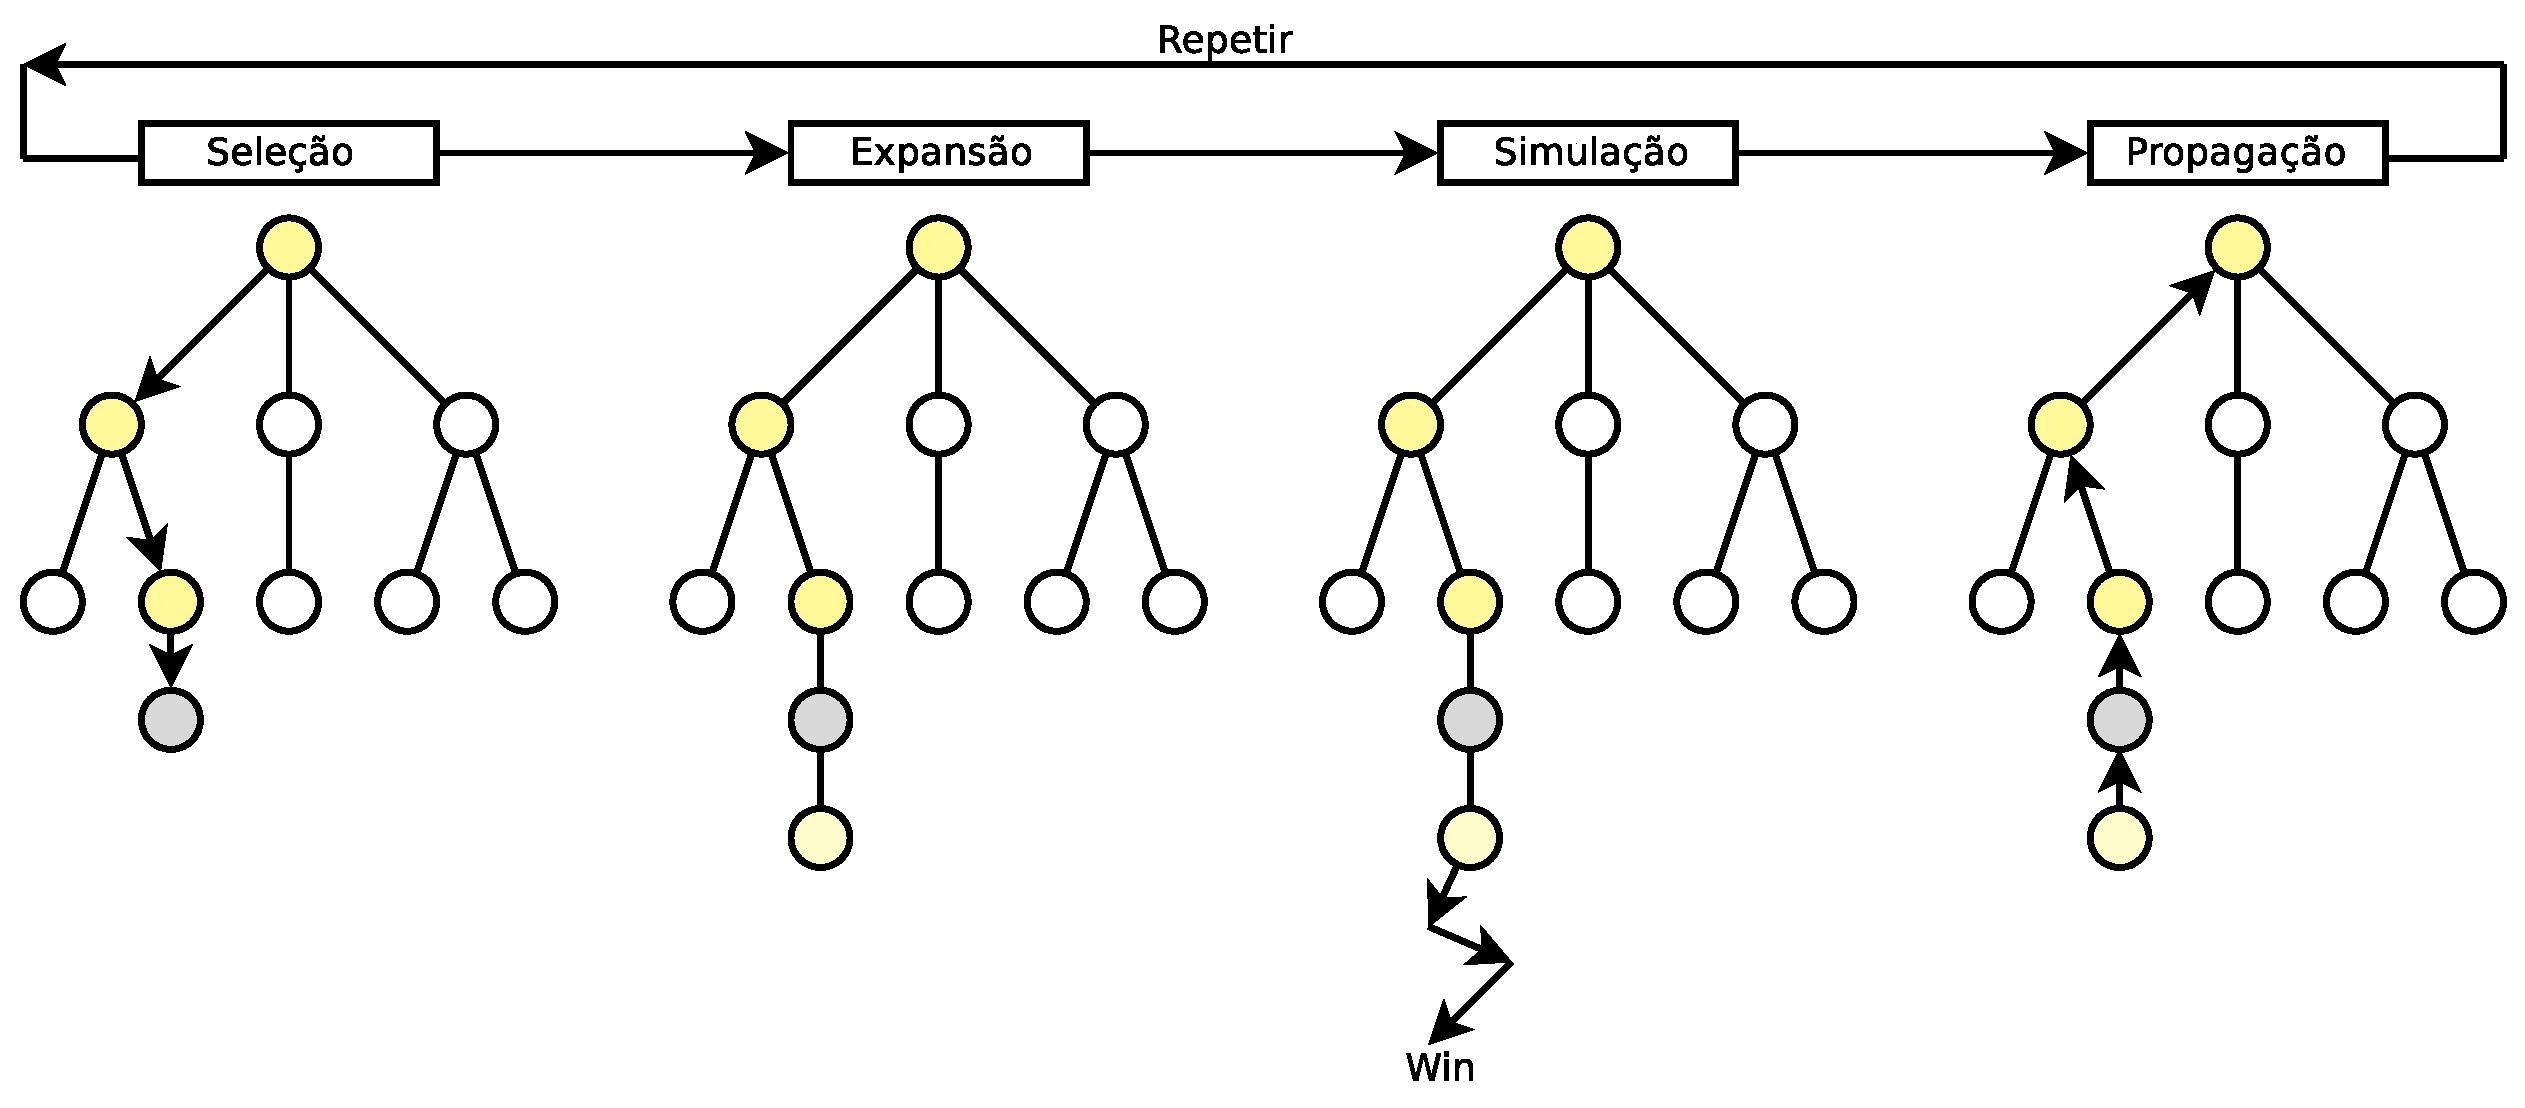
\includegraphics[width=1\textwidth]{mcts}
  \caption{A \textit{Monte Carlo Tree Search}}
  \label{fig:mcts}
\end{figure}

\subsubsection{\textit{Upper Confidence Bound} e o \textit{Multi-Armed Bandit}}

O problema principal do algoritmo anterior está na fase de
Seleção. Como é que se escolhe o próximo nó a explorar? Por um lado
pode ser boa ideia tentar explorar o que nós parece mais promissor de
momento, mas com isto pode-se deixar de lado nós que são muito mais
promissores (ficando preso num máximo local). Por outro lado pode-se
dar prioridade aos nós menos explorados, mas assim não estamos a tirar
partido da informação que vamos tendo (a árvore fica simétrica). Isto
é análogo ao problema clássico do \textit{Multi-Armed Bandit}, onde
dado um conjunto de \textit{slot-machines} com diferentes níveis de
recompensa, como é que se pode obter uma estratégia que maximize os
ganhos do jogo. É o dilema da exploração contra aproveitamento (em
inglês \textit{exploitation vs exploration}).

Existem várias maneiras de abordar este problema. Uma das primeiras a
ser aplicada a \texttt{MCTS} chama-se \textit{Upper Confidence
  Bound}. Este método seleciona cada nó uma vez
inicialmente. Posteriormente usa a seguinte fórmula de exploração e
escolhe o nó que a maximiza: $\bar{X_i} + c
\sqrt{\frac{\log{n}}{n_i}}$ para cada nó $i$, onde $\bar{X_i}$ é o
valor médio desse nó (que no contexto da \texttt{MCTS} é dado pelo
número de vezes que uma simulação a partir desse nó resultou numa
vitória, sobre o número total de vezes que o nó foi escolhido para uma
simulação), $n$ é o número total de vezes que foi efetuada uma seleção
que envolvesse aquele nó (que corresponde ao número de vezes que o pai
desse nó foi selecionado para uma simulação), $n_i$ corresponde ao
número de seleções para simulação desse nó e $c$ é a chamada constante
de \texttt{UCB} e que normalmente é $\sqrt{2}$. À combinação deste
formula com \texttt{MCTS} chama-se de \textit{Upper Confidence bound
  to Trees}. O uso deste método revelou-se muito positivo e desde
então já foi muito estudado e melhorado.

\subsubsection{Heurísticas: \textit{Heavy} e \textit{Light} \textit{Playouts}}

Os métodos descritos até à subsecção anterior constituem a base do que
é a \texttt{MCTS}. Este algoritmo elegante até agora não necessitou de
nenhum conhecimento específico do jogo para o guiar e por isso é um
\textit{General Playing Algorithm}. Porém, para jogos de média
complexidade e alta complexidade, estabiliza em níveis baixos de
desempenho e por isso não é muito competitivo. Por isso, é necessário
aplicar um conjunto de otimizações e técnicas para melhorar a sua
performance. Uma delas é introduzir heurísticas no algoritmo. É
possível introduzir heurísticas em várias das fases do algoritmo, aqui
descrevemos o seu uso na fase de Simulação.

É possível fazer os \textit{playouts} puramente aleatórios e escolher
cada jogada a seguir aleatoriamente. A isto chama-se \textit{light
  playouts}. De um modo geral não funcionam mal, porque
experimentalmente verificou-se que \textit{playouts} de valor inferior
(jogados de maneira mais \textit{naive}) levam a melhores resultados
do método geral (em comparação com métodos não perfeitos, claro que se
o \textit{playout} fosse perfeito o seu resultado dava a informação
completa e não eram necessários mais). Infelizmente, no caso geral são
normalmente necessárias demasiadas iterações para se obter um bom
resultado. Assim, foi introduzido conhecimento especifico do jogo para
guiar os \textit{playouts}. A isto chama-se \textit{heavy playouts}. O
método mais comum e que leva à maior eficiência é o chamado
\textit{Best-of-N}, que corresponde a gerar um conjunto de $N$ jogadas
possíveis em cada turno do \textit{playout} e escolher das $N$ a que
leva a um tabuleiro com valor de heurística superior. A única
desvantagem deste método é que torna a simulação mais lenta e por isso
obriga a diminuir o número de iterações, mas no geral os resultados
melhoram.

\subsubsection{Otimizações Comuns}
\label{sec:mcopt}

%(http://www.arimaa.com/arimaa/papers/ThomasJakl/bc-thesis.pdf Section 3.2)
%(http://arimaa.com/arimaa/papers/TomasKozelekThesis/mt.pdf Section 3.3)

Nesta subsecção introduzimos algumas das otimizações mais comuns e que
levam a melhores resultados com a \texttt{MCTS}. Como o espaço é
limitado (e o tempo também), descrevem-se apenas brevemente cada uma.

\begin{itemize}
\item \textbf{\textit{Progressive Bias}}: Esta otimização corresponde
  combinar informações estimadas com informações empíricas, ao
  introduzir um termo na fórmula de exploração \texttt{UCB} de
  $\frac{H_i}{n_i + 1}$, onde o $H_i$ corresponde a um coeficiente
  obtido a partir da heurística. Assim, a heurística ajuda a guiar
  quais os nós parecem promissores no início, quando ainda foram
  executados poucas iterações;
\item \textbf{\textit{Virtual Visits}}: Corresponde a iniciar o nó com
  um conjunto de visitas (o $n_i$ da fórmula de exploração) positivo,
  assim como número de \textit{playouts} com sucesso (que afeta a
  variável $\bar{X_i}$). Este número de visitas é uma constante $k$ e
  o número de \textit{playouts} com sucesso é dependente da heurística
  e será algo como $H_i * k$ (assumindo a heurística
  normalizada). Assim como a otimização anterior, ajuda a guiar a
  seleção no inicio e introduz algum valor heurístico nos nós;
\item \textbf{\textit{Maturity Threshold}}: Esta pequena otimização
  pode revelar-se muito importante em vários casos. A ideia é limitar
  a expansão de nós, só expandindo nós que já tenham tido pelo menos
  um número de visitas (ou um número de escolhas para simulação) maior
  ou igual a um coeficiente chamado coeficiente de
  maturidade. Normalmente também se usa a profundidade do nó para
  limitar a expansão, que combinado com o coeficiente, ajuda a não
  expandir nós demasiadamente profundos para terem impacto no valor
  dos nós mais superiores;
\item \textbf{\textit{Children Caching}}: Esta otimização pretende
  diminuir o tempo gasto no passo de seleção. A ideia é manter uma
  \textit{cache} com número pequeno de filhos do nó e só selecionar
  nós desta \textit{cache}. A \textit{cache} é preenchida com um
  conjunto dos melhores nós (com valor mais alto da função de
  exploração \texttt{UCB}) e é esvaziada e recalculada de tempo a
  tempo;
\item \textbf{\textit{Grandfather Heuristics}}: Neste otimização
  inicializa-se o número de visitas e o valor do nó com o número de
  visitas e o valor do nó do nó dois níveis acima (o antecessor do
  antecessor), caso exista. A ideia é que se uma jogada foi positiva,
  então a sua continuação também a será;
\item \textbf{\textit{Transposition Tables}}: Esta adaptação da
  otimização já existente na pesquisa \textit{Alpha-Beta} tem como
  objetivo evitar nós com tabuleiros repetidos, fazendo um
  \textit{merge} de nós com o mesmo tabuleiro;
\end{itemize}

Existem muitas mais otimizações e técnicas para melhorar a
\texttt{MCTS}. A mais importante não referida é a chamada
\textit{Rapid Action Value Estimation} que é muito usada em jogos de
colocação de peças (como o \textit{Go}) cujo objetivo é de considerar
a informação que uma jogada teve num \textit{playout} para todos os
tabuleiros que contenham essa jogada.

%----------------------------------------------------------------------------------------
%	SECTION 3
%----------------------------------------------------------------------------------------


\section{O Jogo de Sesqui}
\label{sec:sesqui}

(Porque escolhemos o jogo)

\lipsum[1]

\subsection{Regras do Jogo}

\lipsum[1]

\lipsum[2]

\lipsum[3]

\subsection{Alguns Resultados sobre o Jogo}

(Numero de tabuleiros, empates, vantagem do segundo)

\lipsum[1]

\lipsum[2]

\subsection{Intuição para a Implementação}

\lipsum[1]

\lipsum[2]

%----------------------------------------------------------------------------------------
%	SECTION 4
%----------------------------------------------------------------------------------------

\section{Implementação}
\label{sec:imp}

\lipsum[1]

\subsection{Minimax}

A implementação do algoritmo Minimax é baseada no pseudo-código de Russell\cite{Russell:AI:2003}. Devido ao elevado fator de ramificação do jogo, fomos obrigados a impor limites à pesquisa adversarial Minimax. Atualmente esse limite de profundidade é de 3 \emph{ply}.

Na mesma implementação de Minimax, adicionamos umas cláusulas para permitir \emph{pruning} e efetivamente transformar o algoritmo em \emph{Alpha-Beta Pruning}.

Ao atingir a profundidade máxima permitida, o valor do nó atual é estimado por uma função heurística.

\subsection{\texttt{MCTS}}

\lipsum[1]

\lipsum[2]

\lipsum[3]

\subsection{Heurísticas}

\lipsum[1]

\lipsum[2]

\lipsum[3]

%----------------------------------------------------------------------------------------
%	SECTION 5
%----------------------------------------------------------------------------------------

\section{Resultados e Desempenho}
\label{sec:resdes}

\lipsum[1]

\lipsum[2]

\lipsum[3]

%----------------------------------------------------------------------------------------
%	SECTION 6
%----------------------------------------------------------------------------------------

\section{Conclusão e Trabalho Futuro}
\label{sec:conc}

Paralelismo, Otimizações no AB, MC-AB (juntar os dois)\cite{Dutra:2015}

\lipsum[1]

\lipsum[2]

\bibliographystyle{plain}
\bibliography{lab_report_2}

\end{document}
